% !TEX root = ./proj_report.tex
\graphicspath{{mehul_pics/}}% Set graphics path location

\chapter{Filter Performance}
\noindent {\bf Image processing and degradation model: }\\
Blurred images are modeled as the true image convolved with a point spread function and additive noise. The point spread function (PSF) that convolves the true image is generally a property associated with the optics that have contributed to the blur while noise can be due to poor illuminance, quantization errors and other sources. Mathematically, a blurry image can be represented as follows\\
\begin{equation}
v(m,n)= h(m,n) \star u(m,n) + \eta(m,n)
\end{equation}
where, $u(m,n)$ is the true image, $h(m,n)$ is the PSF, $\eta(m,n)$ is the additive noise and $v(m,n)$ is the blurry image. Image sharpening involves calculating an estimate of the true image $\hat{u}(m,n)$ using filters.
\begin{equation}
\hat{u}(m,n)= g(m,n) \star v(m,n)
\end{equation}
Filters calculate function $g(m,n)$ using some knowledge of the PSF that caused the blur and an estimate of the signal to noise ratio.\\

\noindent {\bf Filter kernels: }\\
Choice of filter is very important in image restoration and retrieved image characteristics. This part of the project aims to study and compare different filters based on enhancement effectiveness and deblur characteristics under various blur sources. Before we present a comparison, let us briefly discuss the different filters studied for the purposes of this project. Various filters compared are, 
\begin{enumerate}
\item Inverse and Pseudo filter
\item Wiener filter
\item Geometric mean filter
\item Constrained least squares filter
\end{enumerate} 
Mathematical formulation of these filters has been presented in the Appendix and will not be discussed here. 
\section{Train Image: Supersonic flow around a sphere}
In this simulated motion blur, train image was procured from Van Dyke's Album of Fluid Motion and depicts the formation of shock around a sphere at flow Mach no. 3. This image was blurred using a motion PSF and had Gaussian white additive noise. The blurred image and recovered image are presented below. Filter deblur characteristics follow below.

\begin{figure}
        \centering
        \begin{subfigure}[b]{0.4\textwidth}
                \centering
                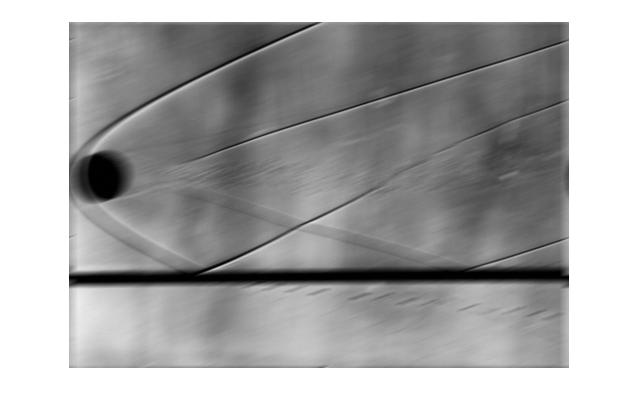
\includegraphics[width=\textwidth]{ssphere_motion.jpg}
                \caption{Blurry image}
                
        \end{subfigure}
        \begin{subfigure}[b]{0.4\textwidth}
                \centering
                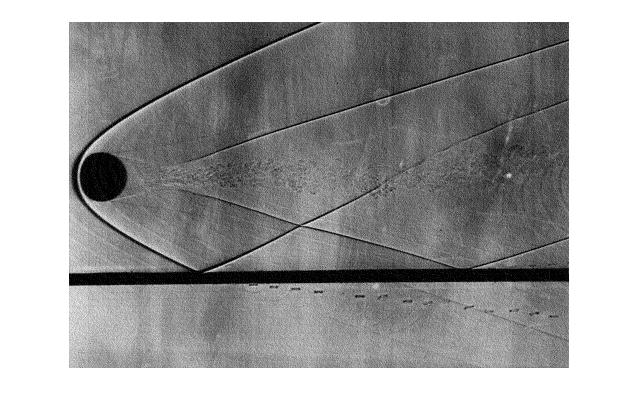
\includegraphics[width=\textwidth]{ssphere_wiener.jpg}
                \caption{Wiener filter sharpened image} 
        \end{subfigure}
\caption{Image enhancement on the blurred image was performed using all the filters. For representative purposes only the sharpened image using Wiener filter has been shown here. Blur PSF used for this simulation represented blur effect due to motion. Variance of the additive noise is of $O(10^{-5}$. }
\end{figure}

\begin{figure}[h!]
  \centering
                \centering
                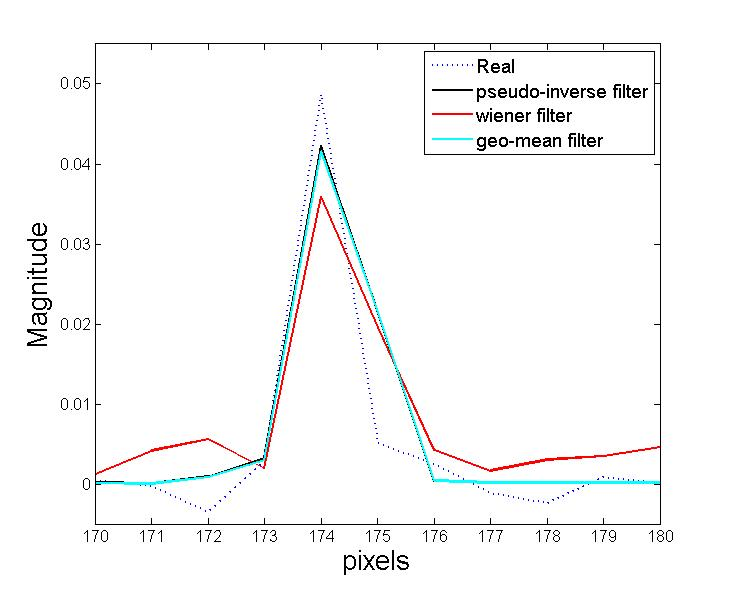
\includegraphics[width=.5\textwidth]{kernel_motion.jpg}
                \caption{Kernel comparison for blur due to motion}
                \end{figure}

\begin{figure}
        \centering
        \begin{subfigure}[b]{0.4\textwidth}
                \centering
                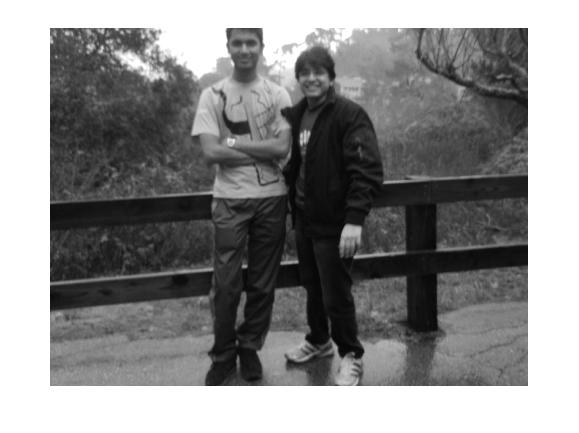
\includegraphics[width=\textwidth]{blur_personal.jpg}
                \caption{No reference blurry image}
                
        \end{subfigure}
        \begin{subfigure}[b]{0.4\textwidth}
                \centering
                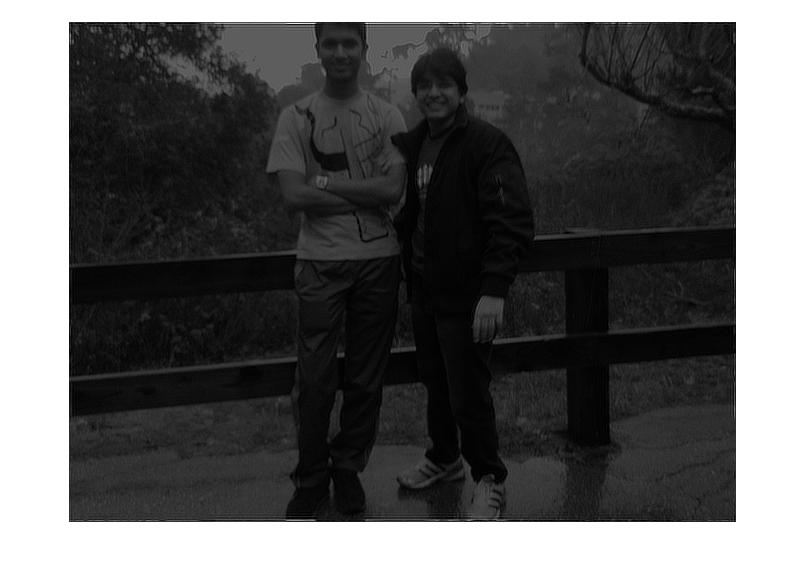
\includegraphics[width=\textwidth]{sharp_personal.jpg}
                \caption{Wiener filter sharpened image} 
        \end{subfigure}
\caption{No reference image enhancement}
\end{figure}

\newpage